% compile this file with xelatex
\documentclass[12pt]{article}
\usepackage{graphicx}
\usepackage[margin=2cm, a4paper]{geometry}
\usepackage{setspace}
\usepackage{pdfpages}
\usepackage{float}
\usepackage{ctex}
\usepackage{amsmath}
\usepackage{fancyvrb}
\usepackage{amssymb}
\usepackage{minted}
\usepackage{enumitem}
\usepackage[colorlinks,linkcolor=blue]{hyperref}

\usepackage{xeCJK}
\setCJKmainfont{Noto Sans TC}

\renewcommand{\contentsname}{Contents}
\renewcommand{\figurename}{Figure}
\renewcommand{\tablename}{Table}
\hypersetup{
    colorlinks=true,
    linkcolor=black,
    filecolor=magenta,      
    urlcolor=blue,
}
\newcommand{\mytitle}{數位影像處理 Homework Assignment \#2}
\newcommand{\myauthor}{B13902022 賴昱錡}

\usepackage{fancyhdr}
\pagestyle{fancy}
\fancyhead{}
\fancyhead[L]{\mytitle}
\fancyhead[R]{\myauthor}

\title{\mytitle}
\author{\myauthor}
\date{}

\begin{document}

\onehalfspacing
\maketitle

\section{Part A}

\newpage
\section{Part B}
\subsection{Source Code}
\subsubsection{Usage}
\begin{Verbatim}[linenos]
python3 HistEqualization.py [*.png or *.jpg]
\end{Verbatim}

One example is \texttt{python3 HistEqualization.py monica.png}, note that the program takes one existing \textbf{png} or \textbf{jpg} file as the only argument

Also, in my program, I use modules like \texttt{opencv, matplotlib, numpy, sys}, so please make sure these modules are installed before running.
\begin{minted}[frame=lines,framesep=2mm,baselinestretch=1.2,linenos,breaklines]{python}
import cv2 as cv
import numpy as np
import sys
import matplotlib.pyplot as plt

assert len(sys.argv) == 2, "The program takes one file as argument!"
assert sys.argv[1].endswith('jpg') or sys.argv[1].endswith('png'), "This is not image file!"

filename = ""

try:
    filename = sys.argv[1]
except:
    print('Please enter filename!')

img = cv.imread(filename)
grey_img = cv.cvtColor(img, cv.COLOR_BGR2GRAY)
equalized_img = cv.equalizeHist(grey_img)

plt.subplot(2, 2, 1)
plt.hist(grey_img.ravel(),256,[0,256]);
plt.ylabel('count of pixels')
plt.xlabel('intensity')
plt.title('Original Greyscale Image')

plt.subplot(2, 2, 2)
plt.hist(equalized_img.ravel(),256,[0,256]);
plt.ylabel('count of pixels')
plt.xlabel('intensity')
plt.title('Histogram Equalized Image')

grey_img = cv.cvtColor(grey_img, cv.COLOR_GRAY2RGB)
plt.subplot(2, 2, 3)
plt.imshow(grey_img)
plt.axis('off')

equalized_img = cv.cvtColor(equalized_img, cv.COLOR_GRAY2RGB)
plt.subplot(2, 2, 4)
plt.imshow(equalized_img)
plt.axis('off')

plt.tight_layout()
plt.show()
\end{minted}
\subsection{Explanation}
Line 1 to line 14 import necessary modules, handle the exception and take one file name as the argument for future processing.

From line 16 to line 18, the program reads the image, and converts the values of the image in BGR color space (a tuple of 3 values, each from 0 to 255) to greyscale space (0 to 255). And then use \texttt{cv2.equalizeHist} to do histogram equalization on this greyscale image.

The rest of the code is about plotting the results of images and histogram of intensity before and after processing in several subplots. The most important part is \texttt{plt.hist(equalized\_img.ravel(),256,[0,256])}, since it flatten the 2-d array of images to 1-d array and put the data into function for making histograms, also, for the proper display of image in matplotlib, we need to convert the pixel data in greyscale space to RGB color space.
\subsection{Demo}
We can clearly find that the histogram-equalized image is brighter (compared to original photo taken in the dark place) and has higher contrast. Also, the distribution of intensity of each pixel is more even, in other words, much flatter, this is what we want from histogram equalization. The picture below is \texttt{demo.png}, it can be displayed again by running command below:
\begin{Verbatim}[linenos]
python3 HistEqualization.py selfie.jpg
\end{Verbatim}
\begin{figure}[H]
    \centering
    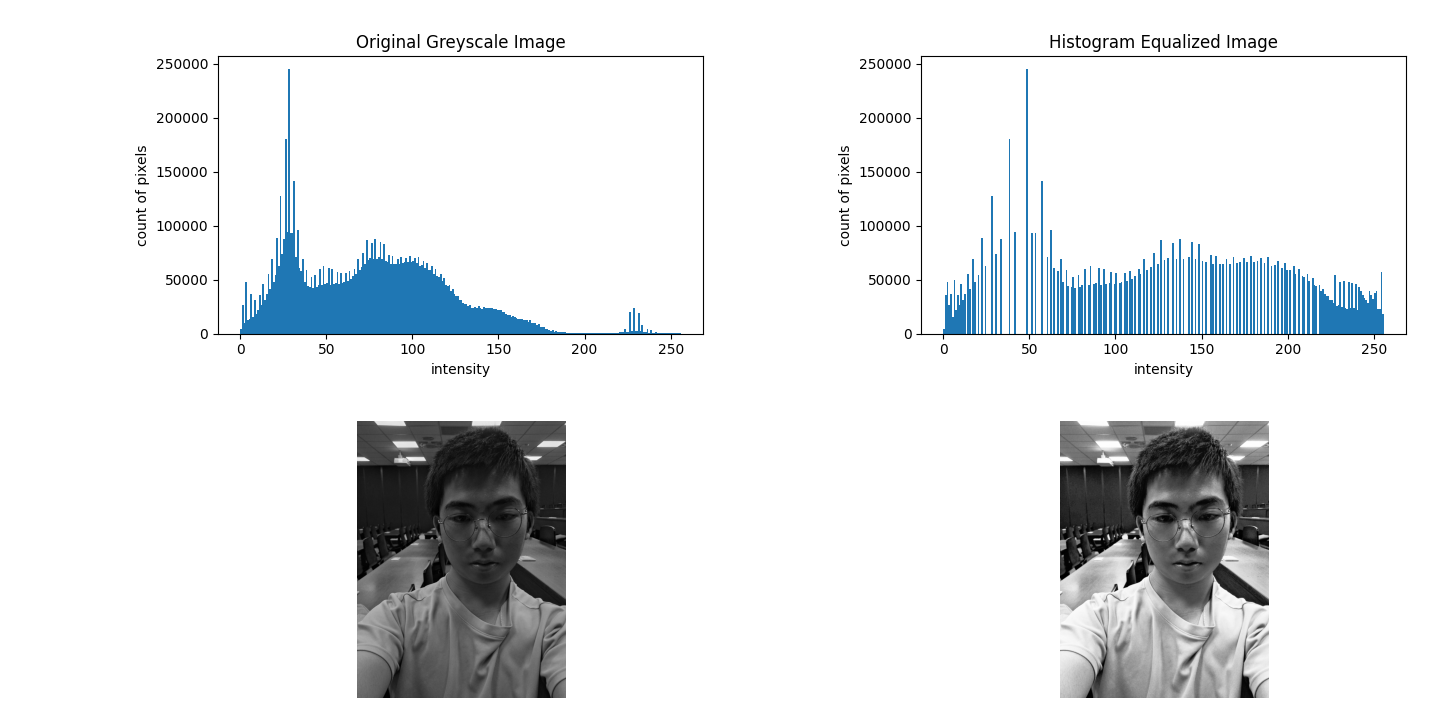
\includegraphics[width=1\linewidth]{demo.png}
    \caption{The histograms and results of my selfie before and after 
histogram equalization}
\end{figure}


\end{document}
% how to display codes?
% \begin{minted}[frame=lines,framesep=2mm,baselinestretch=1.2,linenos,breaklines]{python}
% \end{minted}

% how to display images?
% \begin{figure}[H]
%     \centering
%     \includegraphics[width=0.5\linewidth]{}
%     \caption{Caption}
% \end{figure}
% test